% Copyright (C) 2020 Diogo Rodrigues, Breno Pimentel
% Distributed under the terms of the GNU General Public License, version 3

\documentclass[a4paper, 11pt]{report}
\usepackage[top=35mm,bottom=35mm,left=25mm,right=25mm]{geometry} % Margins

% Change section numbers
\renewcommand{\thesection}{\arabic{section}}

% Second page
\usepackage{secondpage}
\usepackage{datetime}

% Appendix
\usepackage{appendix}

% Landscape pages
\usepackage{pdflscape}

% Decent underlines
\usepackage[normalem]{ulem}

% Hyperreferences
\usepackage{hyperref}

% Imports
\usepackage{import}

% Graphics and images
\usepackage{graphicx} \graphicspath{{./images/}}
\usepackage{tikz}
\usepackage{tikz-qtree}
\usetikzlibrary{automata, positioning, arrows}
\usepackage[justification=centering]{caption}
\usepackage{subcaption}
\usepackage{float}

% Encodings (to render letters with diacritics and special characters)
\usepackage[utf8]{inputenc}

% Language
\usepackage[english]{babel}

% Source code and algorithms
%\usepackage{amsmath}
\usepackage{algorithm}
\usepackage[noend]{algpseudocode}
\usepackage{listings}
\lstset{
	basicstyle=\linespread{0.85}\ttfamily,
	basewidth  = {0.50em,1em},
    frame=tb, % draw frame at top and bottom of the code
    tabsize=4, % tab space width
    numbers=left, % display line numbers on the left
	showstringspaces=false, % don't mark spaces in strings    
    commentstyle=\color{green}, % comment color
    keywordstyle=\color{blue}, % keyword color
	stringstyle=\color{red} % string color
}

% Tables with bold rows
\usepackage{tabularx}
\newcommand\setrow[1]{\gdef\rowmac{#1}#1\ignorespaces}
\newcommand\clearrow{\global\let\rowmac\relax}
\clearrow
\usepackage{multirow}

% Tables with vertical center alignment
\usepackage{array}

% Lists and items
\usepackage{enumitem}

% Math stuff
\usepackage[mathscr]{euscript}
\usepackage{amssymb, latexsym} %Load math symbols like \blacksquare, but also load normal \leadsto arrows
\usepackage{mathtools} % For \text{...}
% \usepackage{enumitem}
% \usepackage{xcolor}
\newcommand{\expnumber}[2]{{#1}\mathrm{e}{#2}} % scientific notation
\usepackage{siunitx} %SI units
\newcommand{\degree}{^{\circ}}
\newcommand*\xor{\oplus}

% Headers and footers
\usepackage{fancyhdr}
\pagestyle{fancyplain}
\fancyhf{}
\lhead{\fancyplain{}{Serial port data protocol — Report (RCOM 2020/21)}}
\rhead{\fancyplain{}{Class 2, group 4}}
\lfoot{\fancyplain{}{\leftmark}}
\rfoot{\thepage}

% Email
\newcommand{\email}[1]{
{\texttt{\href{mailto:#1}{#1}} }
}

% Metadata
\title{\Huge Serial port data protocol \\ \Large Report \\ \vspace*{4pt} \large RCOM 2020/21}
\author{
Class 2, group 4 \vspace{0.5em} \\
\begin{tabular}{r l}
	\email{up201800170@fe.up.pt} & Breno Accioly de Barros Pimentel \\
	\email{up201806429@fe.up.pt} & Diogo Miguel Ferreira Rodrigues  \\
\end{tabular}
}
\date{25th of May, 2020}

% Document
\begin{document}
\maketitle
\begin{secondpage}
    Copyright \copyright 2020--\the\year\ Diogo Rodrigues, Breno Pimentel\par
    \IfFileExists{VERSION}{Version \input{VERSION}}{Draft version}\par
    \immediate\write18{./get-commit-info.sh > COMMIT.tex}
    Built on \today~\currenttime~from \href{https://github.com/dmfrodrigues/feup-rcom-l1}{dmfrodrigues/feup-rcom-l1}, commit \input{COMMIT}\unskip.\par
    Permission is granted to copy and distribute this document under the terms of the
    \href{https://creativecommons.org/licenses/by-nc-nd/4.0/}{Creative Commons Attribution-NonCommercial-NoDerivatives 4.0 International}
    public license.
\end{secondpage}
\clearpage

\pagenumbering{arabic}

\section*{Summary}

This project was elaborated in the context of the curricular unit Computer Networks (\textit{Redes de Computadores} - RCOM) as the first laboratory project. It concerns the design and implementation of a data link layer/protocol to allow two computers to communicate in a reliable way through serial ports. Additionally, an application was developed on top of that layer, to allow a computer to transfer a file to another.

Our main conclusions were...

% TODO

\section{Introduction} \label{sec:Introduction}

The present project aims at arriving at a design and implementation of a data link layer suited with its own data transfer protocol to allow communication between two computers physically connected through RS-232 serial ports with asynchronous communication. The resulting source code was developed in the C language, targetting Linux devices.

This report is an artifact of the corresponding project, with the purpose of guiding readers through the process that was used to arrive at the project's goals. As such, this report is divided into seven main sections (excluding the \hyperref[sec:Introduction]{introduction} and \hyperref[sec:Conclusion]{conclusion}). In section \ref{sec:Architecture} we start by describing the generic architecture our program will follow in terms of layers and generic interfaces between layers, to then specity in section \ref{sec:CodeStructure} which specific layers implement the generic blocks of the previous section, the APIs each block will make available for inter-layer communication, and data structures used in each layer. Specific information for the end user on the main ways to use the program is presented in section \ref{sec:UseCases}. In sections \ref{sec:LLProtocol} and \ref{sec:AppProtocol} we identify the main functional aspects and implementation details of the logical link and application protocols respectively. Finally, in section \ref{sec:Validation} we test the program to validate it in terms of efficacy and robustness in face of errors or faulty communication media, and in section \ref{sec:Efficiency} we statistically describe the protocols' experimental efficiency and compare it to a theoretical Stop\&Wait protocol.

\section{Architecture} \label{sec:Architecture}

First of all, we designed the generic architecture of our system. It essentially consists of a lower, data link layer, which is responsible for dealing with the serial port through its driver and the facilities of abstraction through files/terminals provided by a Linux operating system, providing a simple interface to allow synchronous communication between two computers, allowing to open/close ports and write/read generic data to them, and implementing some sort of error-control method; on top of that lower layer, is a high-level application made of two executable files, \texttt{transmitter} and \texttt{receiver}, which take advantage of the data link layer to transfer a file from the transmitter to the receiver, and provide a simple command line interface to the user.

\begin{figure}[H]
	\centering
	\begin{tikzpicture}[->,>=stealth',node distance=1.4cm,initial text=$ $,]
		\node[align=center, draw, minimum width=7cm, minimum height=1.4cm] (app) {Application};
		\node[align=center, draw, minimum width=7cm, minimum height=1.4cm, fill=black!10, below of=app] (link) {Data link};
		\node[align=center, draw, minimum width=7cm, minimum height=1.4cm, fill=black!20, below of=link] (driver) {Serial port driver \\ {\footnotesize \texttt{/dev/ttyS0}}};
		\node[align=center, draw, minimum width=7cm, minimum height=1.4cm, fill=black!30, below of=driver] (hardware) {Hardware \\ {\footnotesize RS-232 asynchronous serial port}};
		\node[align=center, above of=app] at (0, +0.7) (user){
\includegraphics[scale=0.2]{actor.png}};
	
		\draw   (app) 		edge[align=center, left , bend right=88.5		] node{\small open port \\[-0.2em] \small write to port \\[-0.2em] \small close port} (link)
				(link) 		edge[align=center, right, bend right=88.5		] node{\small read from port} (app)
				(link) 		edge[align=center, left , bend right=88.5		] node{\small \texttt{open} \\[-0.2em] \small \texttt{tcsetattr} \\[-0.2em] \small \texttt{write}} (driver)
				(driver) 	edge[align=center, right, bend right=88.5		] node{\small \texttt{tcgetattr} \\[-0.2em] \small \texttt{read}} (link)
				(user) 		edge[align=center, left , bend right=60			] node{\small file to be transferred} (app)
				(app) 		edge[align=center, right, bend right=60			] node{\small transferred file} (user)
			;
	\end{tikzpicture}
	\caption{Architecture of the program to be developed}
\end{figure}

\section{Code structure} \label{sec:CodeStructure}

\begin{figure}[H]
	\centering
	\begin{tikzpicture}[->,>=stealth',node distance=2cm,initial text=$ $,]
		\node[align=center] at (-4.5, +2.2) (actor-transmitter){
\includegraphics[scale=0.2]{actor.png}};
		\node[align=center] at (+4, +2.2) (actor-receiver)   {
\includegraphics[scale=0.2]{actor.png}};
		\node[align=center, draw, minimum width=5cm, minimum height=1.3cm] at (-4.5, -0.3) (transmitter) {Transmitter \\ \footnotesize \texttt{transmitter} at \texttt{COM1}};
		\node[align=center, draw, minimum width=5cm, minimum height=1.3cm] at (+4, -0.3) (receiver) {Receiver \\ \footnotesize \texttt{receiver} at \texttt{COM2}};
		\node[align=center, draw, minimum width=5cm, minimum height=1.3cm, fill=black!10] at (-4.5, -2.6) (ll-transmitter) {Link Layer (LL) \\ \footnotesize \texttt{status=TRANSMITTER}};
		\node[align=center, draw, minimum width=5cm, minimum height=1.3cm, fill=black!10] at (+4, -2.6) (ll-receiver) {Link Layer (LL) \\ \footnotesize \texttt{status=RECEIVER}};
		\node[align=center, draw, minimum width=5cm, minimum height=1.3cm, fill=black!20] at (-4.5, -5.2) (driver-transmitter) {Serial port driver \\ \footnotesize \texttt{/dev/ttyS0}};
		\node[align=center, draw, minimum width=5cm, minimum height=1.3cm, fill=black!20] at (+4, -5.2) (driver-receiver) {Serial port driver \\ \footnotesize \texttt{/dev/ttyS1}};
		\node[align=center, draw, minimum width=5cm, minimum height=1.3cm, fill=black!30] at (-4.5, -7.2) (port-transmitter) {RS-232 serial port \\ \footnotesize \texttt{COM1}};
		\node[align=center, draw, minimum width=5cm, minimum height=1.3cm, fill=black!30] at (+4, -7.2) (port-receiver) {RS-232 serial port \\ \footnotesize \texttt{COM2}};

		\node[align=right] at (-8.3, -0.3) (app) {Application \\ layer};
		\node[align=right] at (-8.15, -2.6) (ll) {Data link \\ layer};
		\node[align=right] at (-8.25, -5.2) (app) {Serial port \\ drivers};
		\node[align=right] at (-8.2, -7.2) (app) {Hardware};
		
		\path   (-5, -3.25) 	edge[align=center, left		] node{\small \texttt{open}, \texttt{close} \\[-0.2em] \small \texttt{tcsetattr}} (-5, -4.55)
				(+3.5, -3.25) 	edge[align=center, left		] node{\small \texttt{open}, \texttt{close} \\[-0.2em] \small \texttt{tcsetattr}} (+3.5, -4.55)

				(-4, -4.55) 	edge[align=center, right	] node{\small \texttt{tcgetattr}} (-4, -3.25)
				(+4.5, -4.55) 	edge[align=center, right	] node{\small \texttt{tcgetattr}} (+4.5, -3.25)

				(-5, -5.85) 	edge[align=center, left		] node{} (-5, -6.55)
				(+3.5, -5.85) 	edge[align=center, left		] node{} (+3.5, -6.55)

				(-4, -6.55) 	edge[align=center, right	] node{} (-4, -5.85)
				(+4.5, -6.55) 	edge[align=center, right	] node{} (+4.5, -5.85)

				;

		\draw	(actor-transmitter)		edge[								]	node{\small \texttt{./transmitter 1 pinguim.gif}}	(transmitter)
				(receiver)				edge[								]	node{\small \texttt{./receiver 2 pinguim.gif}}	(actor-receiver)

				(transmitter)			edge[dashed, above					] node{\textit{transferring file...}} (receiver)

				(transmitter) 			edge[align=center, right	] node{\small \texttt{llopen}, \texttt{llclose}} (ll-transmitter)
				(receiver) 				edge[align=center, left		] node{\small \texttt{llopen}, \texttt{llclose}} (ll-receiver)

				(ll-transmitter) 		edge[dashed, align=center, above	] node{\small \texttt{llwrite} / \texttt{llread}} (ll-receiver)

				(driver-transmitter) 	edge[dashed, align=center, above	] node{\small \texttt{write} / \texttt{read}} (driver-receiver)

				(port-transmitter) 		edge[-, double, double distance=3pt, align=center, above	] node{\small physical cable} (port-receiver)
			;
	\end{tikzpicture}
	\caption{Specific code structure to be implemented for this project}
\end{figure}

We implemented two layers to satisfy the previously presented architecture: two executable files \texttt{transmitter} and \texttt{receiver} in module \texttt{app} as the application layer, and module \texttt{ll} (Link Layer) as the data link layer.

\subsection{App interface}

The \texttt{app} module makes available two executable files, where \texttt{<COM>} is the communication port to be used (\texttt{COM1} corresponds to \texttt{ttyS0}, \texttt{COM2} to \texttt{ttyS1}, ...), and \texttt{<file>} is a file path:
\begin{itemize}
	\item \texttt{./transmitter <COM> <file>}, to send \texttt{<file>} to port \texttt{<COM>}.
	\item \texttt{./receiver <COM>}, to receive a file from port \texttt{<COM>}.
\end{itemize}

This module takes advantage of the link layer interface to transfer a file in chunks, that should be not too large to reduce the probability of having an error and requiring retransmission, and not too small as the total amount of non-data bytes is proportional to the number of frames.

% TODO: How can I configure transmission from the command line?

\subsection{Link layer interface}

The \texttt{ll} module makes available the following C functions through file \texttt{ll.h}, which are meant to be used by the \texttt{app} module executable files:
\begin{itemize}
	\item \texttt{int llopen(int com, ll\_status\_t status)}, to open serial port \texttt{com} (1 for \texttt{COM1}, 2 for \texttt{COM2}, ...) with a certain \texttt{status} (\texttt{TRANSMITTER} or \texttt{RECEIVER}). Returns the connection ID (which is the file descriptor of the open port) if successful, or -1 if an error occured.
	\item \texttt{int llwrite(int id, const char *buffer, int length)} writes the first \texttt{length} bytes of \texttt{buffer} (up to \texttt{LL\_MAX\_SIZE} bytes) to connection with ID \texttt{id}; returns the number of written bytes, or -1 if an error occured.
	\item \texttt{int llread(int id, char *buffer)} reads from the connection with ID \texttt{id} to \texttt{buffer}; \texttt{buffer} must have a size of at least \texttt{LL\_MAX\_SIZE} bytes.
	\item \texttt{int llclose(int id)} closes connection with ID \texttt{id}.
\end{itemize}

To use these functions, one just needs to allocate the buffers with proper sizes. You can also configure the transmission by using custom values for \texttt{ll\_config}, of type \texttt{ll\_config\_t}.

\begin{table}[H]
	\centering
	\begin{tabular}{l | p{12cm}}
		\hline \hline
		\textbf{Field}           & \textbf{Description} \\ \hline
		\texttt{baud\_rate}      & Number of bits transmitted per second; defaults to 38400. Any number may be specified, but only a few specific baud rates can be used; as such, the baud rate is rounded up to the next allowed baud rate, unless it is above the maximum baud rate, 230400. Is loaded on call to \texttt{llopen}. \\ \hline
		\texttt{timeout}         & Time the transmitter waits before retransmitting a message that the receiver did not acknowledge. It is measured in integer seconds, and is than zero. By default it is 3 seconds, and can be set at any time. \\ \hline
		\texttt{retransmissions} & Number of times a frame will be retransmitted before giving up and terminating the connection. Defaults to 3, and can be set at any time. \\ \hline
		\texttt{verbosity}       & If the program is compiled in debug mode, logs will be printed if they are less or as verbose as the value of this field.\\ \hline \hline
	\end{tabular}
	\caption{Fields of \texttt{ll\_config\_t}, and their descriptions}
\end{table}

\section{Main use cases} \label{sec:UseCases}

Assuming \texttt{COM11} of the transmitter computer and \texttt{COM12} of the receiver computer are connected.

\subsection{App programs}

First, start the receiver and connect it to \texttt{COM12} to read the file by calling

\begin{lstlisting}[frame=none, numbers=none]
./receiver 12
\end{lstlisting}
Then, start the transmitter and connect it to \texttt{COM11} to write file \texttt{pinguim.gif} by calling

\begin{lstlisting}[frame=none, numbers=none]
./transmitter 11 pinguim.gif
\end{lstlisting}
	
\subsection{Link Layer (LL)}

To read from serial port \texttt{COM12}/\texttt{ttyS11}:
\begin{enumerate}
	\item Open the serial port with \texttt{id = llopen("/dev/ttyS11", RECEIVER)}.
	\item Allocate \texttt{buffer} with at least \texttt{LL\_MAX\_SIZE} bytes, and read data with \texttt{llread(id, buffer)}.
	\item Close the serial port with \texttt{llclose(id)}.
\end{enumerate}
To write to serial port \texttt{COM11}/\texttt{ttyS10}:
\begin{enumerate}
	\item Open the serial port with \texttt{id = llopen("/dev/ttyS10", TRANSMITTER)}.
	\item Write data with \texttt{llwrite(id, buffer, length)}.
	\item Close the serial port with \texttt{llclose(id)}.
\end{enumerate}

For one call to \texttt{llopen} or \texttt{llclose} in the transmitter, there must be exactly one corresponding call in the receiver; additionally, for each call to \texttt{llwrite} in the transmitter there must be exactly one corresponding call to \texttt{llread} in the receiver. Although it is possible to swap roles (the transmitter can read, and the receiver can write) as-is, it is not advised and will currently return an error to prevent misusage.

\section{Logical link protocol} \label{sec:LLProtocol}

The link layer uses a logical link protocol that applies the automatic repeat request method for error-control, which consists of a transfer-acknowledgement process where the receiver only evaluates the consistency of a frame and does not try to correct it; instead it asks the transmitter to retransmit the whole frame. More specifically, a form of \texttt{stop-and-wait} was implemented, in which a frame is only sent after the previous frame was sent and the respective acknowledgement was received. This allows synchronous communication over an unreliable transfer media.

Communication through this protocol is done by \textit{framing} messages in three types of frames: supervisory frames (S-frames), which are used to supervise the communication; unnunbered frames (U-frames), which are used for other miscellaneous purposes, including to acknowledge the reception of a frame; and information frames (I-frames), which contain the actual data to be transferred, Figure \ref{fig:frames}. In particular, S-frames are used to transmit SET (set up), DISC (disconnect), RR (receiver ready) and REJ (rejected) commands, and U-frames for UA (unnumbered acknowledgement).

\begin{figure}[H]
	\centering
	\begin{tabular}{c p{8mm} c}
		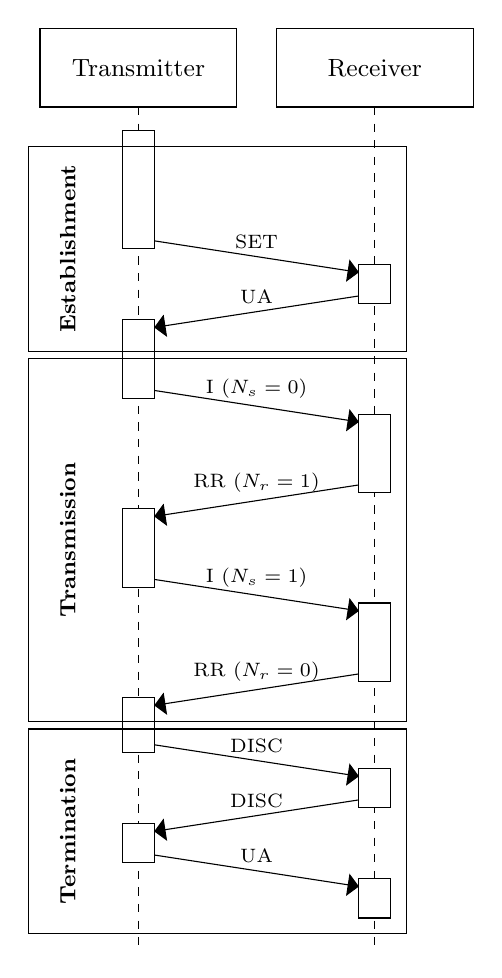
\begin{tikzpicture}[-triangle 90,>=stealth',node distance=2cm,initial text=$ $,]
			\scriptsize
			\node[align=center, draw, minimum width=2.5cm, minimum height=1cm] at (-1.5, 0.8) (transmitter) {\small Transmitter};
			\node[align=center, draw, minimum width=2.5cm, minimum height=1cm] at (+1.5, 0.8) (receiver)    {\small Receiver};
			\node[align=center] at (-2.4, -1.5) (establishment) {\footnotesize \textbf{\rotatebox{90}{Establishment}}};
			\node[align=center] at (-2.4, -5.2) (establishment) {\footnotesize \textbf{\rotatebox{90}{Transmission}}};
			\node[align=center] at (-2.4, -8.9) (establishment) {\footnotesize \textbf{\rotatebox{90}{Termination}}};

			\path 	(-1.5, +0.3) edge[-, dashed] node{} ++(0, -10.7)
					(+1.5, +0.3) edge[-, dashed] node{} ++(0, -10.7);


			\draw [fill = white]
					(-1.7, -0.0) rectangle ++(0.4, -1.5)
					(+1.3, -1.7) rectangle ++(0.4, -0.5)
					(-1.7, -2.4) rectangle ++(0.4, -1.0)
					(+1.3, -3.6) rectangle ++(0.4, -1.0)
					(-1.7, -4.8) rectangle ++(0.4, -1.0)
					(+1.3, -6.0) rectangle ++(0.4, -1.0)
					(-1.7, -7.2) rectangle ++(0.4, -0.7)
					(+1.3, -8.1) rectangle ++(0.4, -0.5)
					(-1.7, -8.8) rectangle ++(0.4, -0.5)
					(+1.3, -9.5) rectangle ++(0.4, -0.5)
					;

			\draw
					(-2.9, -0.2) rectangle (1.9, - 2.8)
					(-2.9, -2.9) rectangle (1.9, - 7.5)
					(-2.9, -7.6) rectangle (1.9, -10.2)
					;
			
			\path
					(-1.3, -1.4)	edge[above]	node{SET} 				++(+2.6, -0.4)
					(+1.3, -2.1)	edge[above]	node{UA}  				++(-2.6, -0.4)
					(-1.3, -3.3)	edge[above]	node{I ($N_s = 0$)} 	++(+2.6, -0.4)
					(+1.3, -4.5)	edge[above]	node{RR ($N_r = 1$)}	++(-2.6, -0.4)
					(-1.3, -5.7)	edge[above]	node{I ($N_s = 1$)} 	++(+2.6, -0.4)
					(+1.3, -6.9)	edge[above]	node{RR ($N_r = 0$)} 	++(-2.6, -0.4)
					(-1.3, -7.8)	edge[above]	node{DISC} 				++(+2.6, -0.4)
					(+1.3, -8.5)	edge[above]	node{DISC} 				++(-2.6, -0.4)
					(-1.3, -9.2)	edge[above]	node{UA} 				++(+2.6, -0.4)
					;

		\end{tikzpicture} & &
		\begin{tikzpicture}[-triangle 90,>=stealth',node distance=2cm,initial text=$ $,]
			\scriptsize
			\node[align=center, draw, minimum width=2.5cm, minimum height=1cm] at (-1.5, 0.8) (transmitter) {\small Transmitter};
			\node[align=center, draw, minimum width=2.5cm, minimum height=1cm] at (+1.5, 0.8) (receiver)    {\small Receiver};

			\node[] at (+0.2, -1.2) (lightning-1)    {
\includegraphics[scale=0.015]{lightning.png}};
			\node[] at (-0.2, -5.4) (lightning-2)    {
\includegraphics[scale=0.015]{lightning.png}};

			\node[align=center] at (+2.6, -7.7) (discarded) {Data \\ discarded \\ (already \\ received)};
	
			\path 	(-1.5, +0.3) edge[-, dashed] node{} ++(0, -10.7)
					(+1.5, +0.3) edge[-, dashed] node{} ++(0, -10.7);
	
	
			\draw [fill = white]
					(-1.7, -0.0) rectangle ++(0.4, -1.0)

					(-1.7, -3.0) rectangle ++(0.4, -1.0)
					(+1.3, -4.2) rectangle ++(0.4, -1.0)

					(-1.7, -6.0) rectangle ++(0.4, -1.0)
					(+1.3, -7.2) rectangle ++(0.4, -1.0)
					(-1.7, -8.4) rectangle ++(0.4, -1.0)
					
					;
			
			\path
					(-1.3, -0.9)	edge[above right]	node{I ($N_s = 0$)} 	++(+1.3, -0.2)

					(-1.3, -3.9)	edge[above		]	node{I ($N_s = 0$)} 	++(+2.6, -0.4)
					(+1.3, -5.1)	edge[above left	]	node{RR ($N_r = 1$)} 	++(-1.3, -0.2)

					(-1.3, -6.9)	edge[above		]	node{I ($N_s = 0$)} 	++(+2.6, -0.4)
					(+1.3, -8.1)	edge[above 		]	node{RR ($N_r = 1$)} 	++(-2.6, -0.4)
					;
	
			\path
					(-2.15, -0.0)	edge[-				]	node{}					(-1.85, -0.0)
					(-2.0, -0.0)	edge[<->, left		]	node{\rotatebox{90}{timeout}}			(-2.0, -3.0)
					(-2.15, -3.0)	edge[-				]	node{}					(-1.85, -3.0)
					(-2.0, -3.0)	edge[<->, left		]	node{\rotatebox{90}{timeout}}			(-2.0, -6.0)
					(-2.15, -6.0)	edge[-				]	node{}					(-1.85, -6.0)
					;

		\end{tikzpicture} \\
		(\textit{a}) & & (\textit{b})
	\end{tabular}
	\caption{Sequence diagrams of communication through the LL protocol: \\ (\textit{a}) complete diagram without errors; (\textit{b}) transmission phase with errors}
	\label{fig:diagrams}
\end{figure}

This protocol is suited with a mechanism that allows the receiver to identify if the arriving frame is a retransmission or not: the sequence number. It is a single bit, referred to as $N_s$ when it is sent by the sender, and $N_r$ when sent by the receiver. It is sent along with I-frames, and when $N_s=0$ the response must have $N_r = 1$, and when $N_s = 1$, $N_r = 0$.  

\begin{figure}[H]
	\centering
	\begin{tabular}{m{6mm} m{108mm}}
		(\textit{a}) & 
		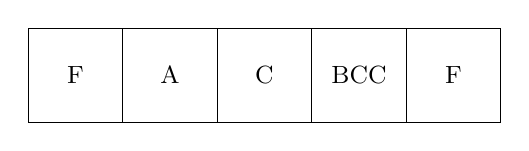
\begin{tikzpicture}[->,>=stealth',node distance=2cm,initial text=$ $,]
			\small
			\node[align=center, draw, minimum width=1.2cm, minimum height=1.2cm] at (0, 0) (f-start) {F};
			\node[align=center, draw, minimum width=1.2cm, minimum height=1.2cm] at (1.2, 0) (a) {A};
			\node[align=center, draw, minimum width=1.2cm, minimum height=1.2cm] at (2.4, 0) (c) {C};
			\node[align=center, draw, minimum width=1.2cm, minimum height=1.2cm] at (3.6, 0) (bcc) {BCC};
			\node[align=center, draw, minimum width=1.2cm, minimum height=1.2cm] at (4.8, 0) (f-end) {F};
		\end{tikzpicture}\\[10pt]
		(\textit{b}) & 
		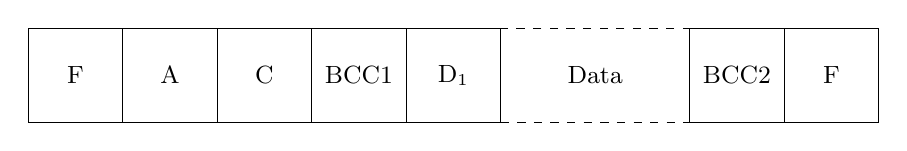
\begin{tikzpicture}[->,>=stealth',node distance=2cm,initial text=$ $,]
			\small
			\node[align=center, draw, minimum width=1.2cm, minimum height=1.2cm] at (0, 0) (f-start) {F};
			\node[align=center, draw, minimum width=1.2cm, minimum height=1.2cm] at (1.2, 0) (a) {A};
			\node[align=center, draw, minimum width=1.2cm, minimum height=1.2cm] at (2.4, 0) (c) {C};
			\node[align=center, draw, minimum width=1.2cm, minimum height=1.2cm] at (3.6, 0) (bcc) {BCC1};
			\node[align=center, draw, minimum width=1.2cm, minimum height=1.2cm] at (4.8, 0) (d1) {D$_1$};
			\node[align=center, dashed, draw, minimum width=2.4cm, minimum height=1.2cm] at (6.6, 0) (data) {Data};
			\node[align=center, draw, minimum width=1.2cm, minimum height=1.2cm] at (8.4, 0) (bcc2) {BCC2};
			\node[align=center, draw, minimum width=1.2cm, minimum height=1.2cm] at (9.6, 0) (f-end) {F};
		\end{tikzpicture}
	\end{tabular}
	\caption{Structure of the S/U-frames (\textit{a}) and I-frames (\textit{b}). Each square represents a byte, which can be F (flag), A (address), C (control), BCC (block check character) or D (data).}
	\label{fig:frames}
\end{figure}

The meaning of the constituents of frames are as follows:

\begin{itemize}
	\item Flag (F, FLAG, \texttt{0x7E}): marks the beginning and end of a frame.
	\item Address (A): identifier of the sender, or of the destination if it is an answer. Takes values \texttt{0x03} for the transmitter and \texttt{0x01} for the receiver.
	\item Control (C): identifies the command; \texttt{0x03} for SET, \texttt{0x0B} for DISC, \texttt{0x07} for UA, \texttt{0b0S000000} for I, \texttt{0bR0000101} for RR and \texttt{0bR0000001} for REJ, where $\texttt{S} = N_s$ and $\texttt{R} = N_r$.
	\item Block check character (BCC): exclusive-or ($\xor$) of a certain range of bytes; BCC and BCC1 are $\text{A}\xor\text{C}$, and BCC2 is $\text{D}_1 \xor \text{D}_2 \xor ... \xor \text{D}_\text{N}$. Is used to check for bit swaps.
	\item Data (D): data bytes, encoded using byte stuffing.
\end{itemize}

Frame reception was implemented using state machines. S-frame and U-frame reception was implemented using the same automaton, as they contain the same number and type of fields; it saves the state, as well as the most recently read values of A and C. I-frames were implemented using a different automaton, as there was no need for storing the values of A and C (which could be directly checked by the automaton), and it additionally required a buffer to store read data, so that data could be provided to the caller once the automaton arrived at the Stop state.

% TODO automata figures?
% In appendices

\subsection{Byte stuffing}

We applied the byte stuffing encoding method suggested in the project guidelines, which consists of defining an escape byte ESC (\texttt{0x7E}), and if character $c$ is equal to FLAG or ESC it is replaced by ESC followed by $c' = c \xor \texttt{0x20}$; the result can be easily decoded, since all we have to do is, on finding ESC, decode $c'$ by applying $c' \xor \texttt{0x20} = c \xor \texttt{0x20} \xor \texttt{0x20} = c \xor \texttt{0x00} = c$. This allows to disambiguate the possible situation where a data byte could be confused with FLAG/end of frame.

There is an additional issue, which was not mentioned in the guidelines: BCC2 can also take the same value as FLAG, if the data is for instance \texttt{0x70 0x0E}, in which case there is no way to distinguish BCC2 from FLAG. We have thus decided to extend byte stuffing encoding to BCC2.

\section{Application protocol} \label{sec:AppProtocol}

\section{Validation} \label{sec:Validation}

\section{Efficiency of the data link protocol} \label{sec:Efficiency}

\subsection{Definitions}

\begin{center}
	\small
	\begin{tabular}{c | l | p{84mm} | c}
		\hline \hline
		\textbf{Acronym} & \textbf{Name}                & \textbf{Definition}                              & I/O \\ \hline
		$a$              & Norm. prop. time             & $a = T_{prop}/T_f$                               &     \\
		$T_{prop}$       & Propagation time             & Time for a signal to propagate through the cable &     \\
		$T_f$            & Frame time                   & Time to transfer a frame                         &     \\
		$T$              & Total execution time         & Total execution time of the transmitter          & O   \\
		$L$              & Total messages length        & Total message length, including retransmissions  & I   \\
		$L_f$            & File length                  & Message length excluding retransmissions         & I   \\
		$N$				 & \# of frames                 & Number of actually transferred frames            & I   \\
		$N_e$            & \# of frames with errors     & Frames with errors, inc. during establishment    & I   \\
		$R_e$            & Frame error rate             & Frames with errors per total frame number        &     \\
		$p_e$            & Frame error probability      & Estimated from $R_e$                             &     \\
		$C$              & Capacity                     & Capacity of the system (baud rate)               & I   \\
		$R$              & Data rate                    & Global data transfer rate                        &     \\
		\hline \hline
	\end{tabular}
\end{center}

\begin{equation*}
	a = \frac{TC}{2L} - \frac{1}{2}
\end{equation*}

\begin{equation*}
	R_e = \frac{N}{N_e}
\end{equation*}

\begin{equation*}
	S = \frac{L_f}{T C}
\end{equation*}

\section{Efficiency}

We can determine the efficiency $S$ by using 
\begin{equation} \label{eq:S}
	S = \frac{R}{C}
\end{equation}
where $R$ is the data transfer rate,
\begin{equation} \label{eq:R}
	R = \frac{L_f}{T}
\end{equation}
and as such equation \ref{eq:S} becomes
\begin{equation} \label{eq:S2}
	S = \frac{L_f}{T C}
\end{equation}
and as such we can determine $S$ by varying $L$ and $C$ and measure $T$.

\section{Conclusion} \label{sec:Conclusion}

\pagebreak

\appendix
\appendixpage
\addappheadtotoc
\chapter{Source code}

The source code of this project can be obtained from \href{https://github.com/dmfrodrigues/feup-rcom-l1}{github.com/dmfrodrigues/feup-rcom-l1}. The source code is made available by \textcopyright~Diogo Rodrigues and Breno Pimentel under the \href{https://www.gnu.org/licenses/gpl-3.0.en.html}{GNU General Public License v3} (GPLv3), which you should have received together with the source code, or that you can otherwise obtain online.

During project development and evaluation the repository remained private, although it can be shared with evaluators on request to clarify the development process or due to other justifiable reasons. It will be made public once all equivalent curricular unit projects have been evaluated in the present school year.

% TODO: files

\newgeometry{top=24mm,bottom=24mm,left=14mm,right=14mm}
\fancyhfoffset[E,O]{0pt}

\section{Link Layer (LL)}
\lstinputlisting[caption=\texttt{ll.h}, language=C]{../../include/ll.h}
\lstinputlisting[caption=\texttt{ll.c}, language=C]{../../src/ll.c}

\subsection{Internal code}
\lstinputlisting[caption=\texttt{ll\_internal.h}, language=C]{../../include/ll_internal.h}
\lstinputlisting[caption=\texttt{ll\_internal.c}, language=C]{../../src/ll_internal.c}

\subsection{Utilities}
\lstinputlisting[caption=\texttt{ll\_utils.h}, language=C]{../../include/ll_utils.h}
\lstinputlisting[caption=\texttt{ll\_utils.c}, language=C]{../../src/ll_utils.c}

\begin{landscape}
\subsection{Flags}
\lstinputlisting[caption=\texttt{ll\_flags.h}, language=C]{../../include/ll_flags.h}
\end{landscape}

\subsection{S-frame state machine}
\lstinputlisting[caption=\texttt{ll\_s\_statemachine.h}, language=C]{../../include/ll_s_statemachine.h}
\lstinputlisting[caption=\texttt{ll\_s\_statemachine.c}, language=C]{../../src/ll_s_statemachine.c}

\subsection{U-frame state machine}
\lstinputlisting[caption=\texttt{ll\_u\_statemachine.h}, language=C]{../../include/ll_u_statemachine.h}
\lstinputlisting[caption=\texttt{ll\_u\_statemachine.c}, language=C]{../../src/ll_u_statemachine.c}

\subsection{I-frame state machine}
\lstinputlisting[caption=\texttt{ll\_i\_statemachine.h}, language=C]{../../include/ll_i_statemachine.h}
\lstinputlisting[caption=\texttt{ll\_i\_statemachine.c}, language=C]{../../src/ll_i_statemachine.c}

\section{Application}
\lstinputlisting[caption=\texttt{application\_layer.h}, language=C]{../../include/app.h}
\lstinputlisting[caption=\texttt{application\_layer.c}, language=C]{../../src/app.c}
\lstinputlisting[caption=\texttt{application\_layer.h}, language=C]{../../include/app_args.h}
\lstinputlisting[caption=\texttt{application\_layer.c}, language=C]{../../src/app_args.c}
\lstinputlisting[caption=\texttt{transmitter.c}, language=C]{../../src/transmitter.c}
\lstinputlisting[caption=\texttt{receiver.c}, language=C]{../../src/receiver.c}

\restoregeometry

\chapter{State machines}
\section{U-frame state machine}

A U-frame state machine must be ready to handle the following scenarios:
\begin{itemize}
	\item \textbf{Left:} A correct U-frame;
	\item \textbf{Right:} A retransmitted S-frame (DISC), because if the receiver receives a DISC, but its own DISC is not received by transmitter, then the transmitter will retransmit the first DISC although the receiver was expecting a UA. Must send DISC.
\end{itemize}

\begin{center}
	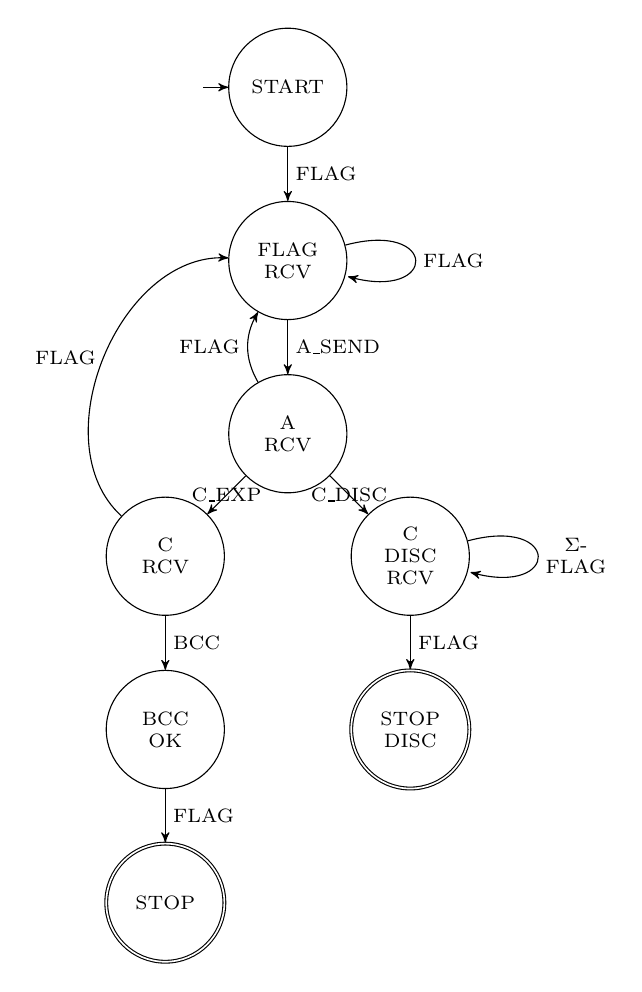
\begin{tikzpicture}[->,>=stealth',node distance=2.2cm,initial text=$ $,state/.style={circle, draw, minimum size=15mm}]
		\scriptsize
		\node[align=center, state, initial								] (START) 		{START};
		\node[align=center, state, below of=START						] (FLAG_RCV) 	{FLAG\\RCV};
		\node[align=center, state, below of=FLAG_RCV					] (A_RCV) 		{A\\RCV};
		\node[align=center, state, below left of=A_RCV					] (C_RCV) 		{C\\RCV};
		\node[align=center, state, below of=C_RCV						] (BCC_OK) 		{BCC\\OK};
		\node[align=center, state, below of=BCC_OK, accepting			] (STOP) 		{STOP};

		\node[align=center, state, below right of=A_RCV					] (C_DISC_RCV) 		{C\\DISC\\RCV};
		\node[align=center, state, below of=C_DISC_RCV, accepting		] (STOP_DISC) 		{STOP\\DISC};

		\draw	(START)			edge[right						]	node{FLAG}		(FLAG_RCV)
				(FLAG_RCV)		edge[loop right					]	node{FLAG}		(FLAG_RCV)
				(FLAG_RCV)		edge[right						]	node{A\_SEND}	(A_RCV)
				(A_RCV)			edge[bend left, left			]	node{FLAG}		(FLAG_RCV)
				(A_RCV)			edge[							]	node{C\_EXP}	(C_RCV)
				(C_RCV)			edge[bend left=70, left			]	node{FLAG}		(FLAG_RCV)
				(C_RCV)			edge[right						]	node{BCC}		(BCC_OK)
				(BCC_OK)		edge[right						]	node{FLAG}		(STOP)

				(A_RCV)			edge[							]	node{C\_DISC}	(C_DISC_RCV)
				(C_DISC_RCV)	edge[align=center, loop right	]	node{$\Sigma$-\\FLAG}	(C_DISC_RCV)
				(C_DISC_RCV)	edge[right						]	node{FLAG}		(STOP_DISC)
				;
		
	\end{tikzpicture}
\end{center}

\newpage
\section{S-frame state machine}

A S-frame state machine must be ready to handle the following scenarios:
\begin{itemize}
	\item \textbf{Left:} A correct S-frame;
	\item \textbf{Right:} A retransmitted I-frame, in case it is expecting DISC but the transmitter was not properly acknowledged that the last I-frame was transmitted. Must send RR.
\end{itemize}

\begin{center}
	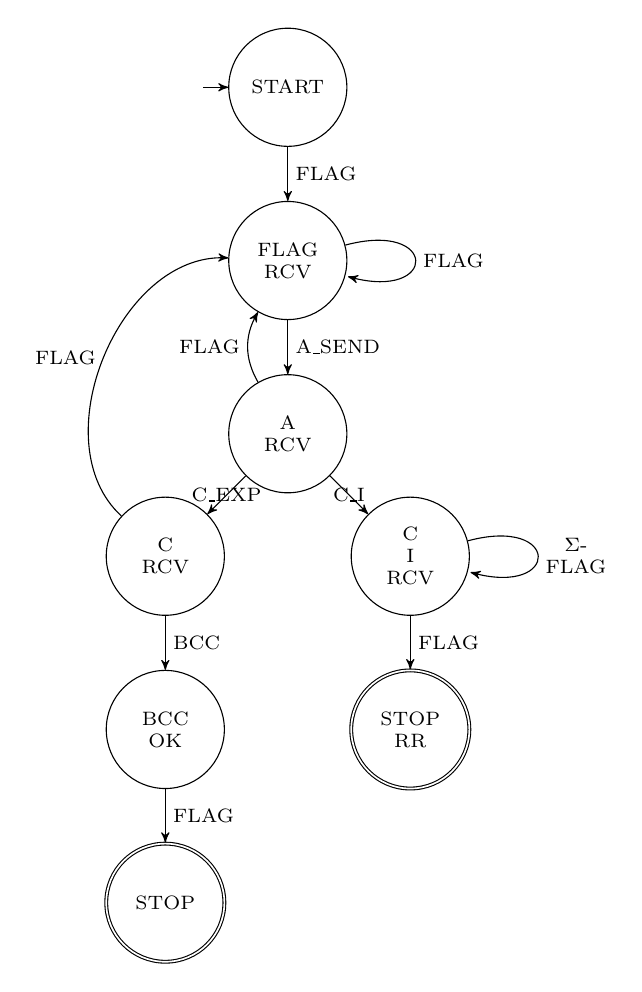
\begin{tikzpicture}[->,>=stealth',node distance=2.2cm,initial text=$ $,state/.style={circle, draw, minimum size=15mm}]
		\scriptsize
		\node[align=center, state, initial								] (START) 		{START};
		\node[align=center, state, below of=START						] (FLAG_RCV) 	{FLAG\\RCV};
		\node[align=center, state, below of=FLAG_RCV					] (A_RCV) 		{A\\RCV};
		\node[align=center, state, below left of=A_RCV					] (C_RCV) 		{C\\RCV};
		\node[align=center, state, below of=C_RCV						] (BCC_OK) 		{BCC\\OK};
		\node[align=center, state, below of=BCC_OK, accepting			] (STOP) 		{STOP};

		\node[align=center, state, below right of=A_RCV					] (C_I_RCV) 		{C\\I\\RCV};
		\node[align=center, state, below of=C_I_RCV, accepting			] (STOP_RR) 		{STOP\\RR};

		\draw	(START)			edge[right						]	node{FLAG}		(FLAG_RCV)
				(FLAG_RCV)		edge[loop right					]	node{FLAG}		(FLAG_RCV)
				(FLAG_RCV)		edge[right						]	node{A\_SEND}	(A_RCV)
				(A_RCV)			edge[bend left, left			]	node{FLAG}		(FLAG_RCV)
				(A_RCV)			edge[							]	node{C\_EXP}	(C_RCV)
				(C_RCV)			edge[bend left=70, left			]	node{FLAG}		(FLAG_RCV)
				(C_RCV)			edge[right						]	node{BCC}		(BCC_OK)
				(BCC_OK)		edge[right						]	node{FLAG}		(STOP)

				(A_RCV)			edge[							]	node{C\_I}		(C_I_RCV)
				(C_I_RCV)		edge[align=center, loop right	]	node{$\Sigma$-\\FLAG}	(C_I_RCV)
				(C_I_RCV)		edge[right						]	node{FLAG}		(STOP_RR)
				;
		
	\end{tikzpicture}
\end{center}

\newpage
\section{I-frame state machine}

An I-frame state machine must be ready to handle to following scenarios:
\begin{itemize}
	\item \textbf{Left:} A correct I-frame;
	\item \textbf{Center:} A retransmitted wrong I-frame. Must ignore the data and respond with RR;
	\item \textbf{Right:} A retransmitted S-frame (SET), as it may be expecting an I-frame but might get a retransmission of a SET from establishment. Must respond with UA.
\end{itemize}

\begin{center}
	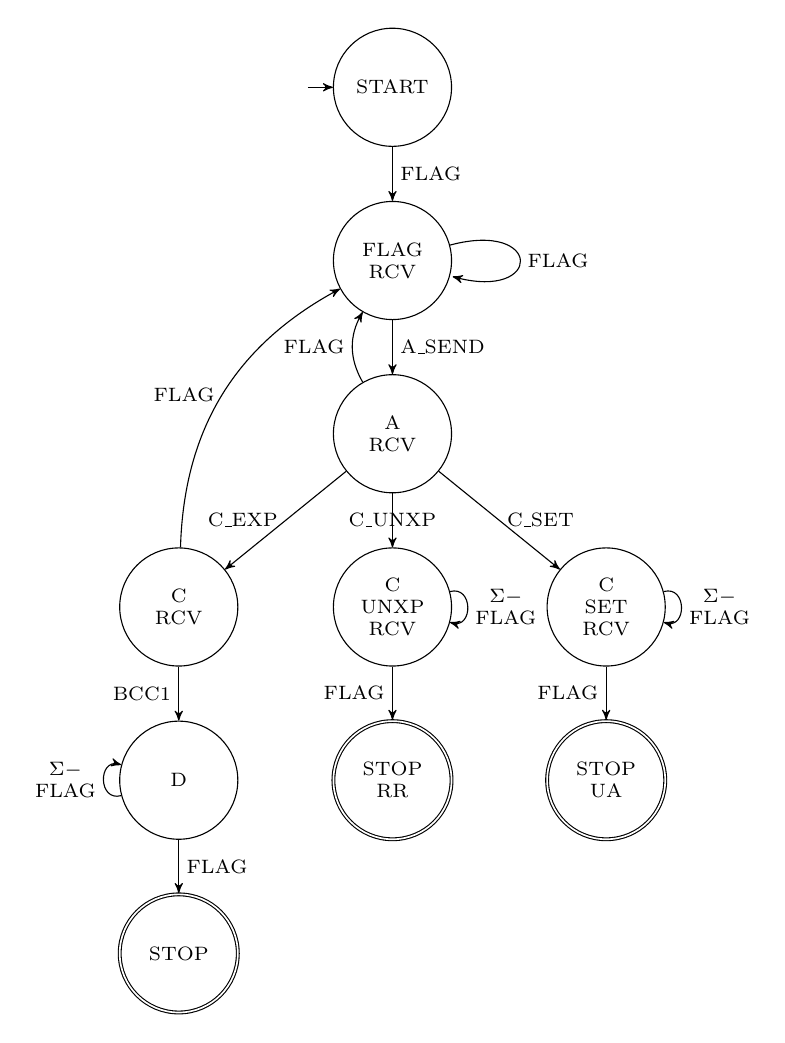
\begin{tikzpicture}[->,>=stealth',node distance=2.2cm,initial text=$ $,state/.style={circle, draw, minimum size=15mm}]
		\scriptsize
		\node[align=center, state, initial								] (START) 		{START};
		\node[align=center, state, below of=START						] (FLAG_RCV) 	{FLAG\\RCV};
		\node[align=center, state, below of=FLAG_RCV					] (A_RCV) 		{A\\RCV};
		\node[align=center, state, below of=A_RCV						] (C_UNXP_RCV)	{C\\UNXP\\RCV};
		\node[align=center, state, left=1.2cm of C_UNXP_RCV				] (C_RCV) 		{C\\RCV};
		\node[align=center, state, below of=C_RCV						] (D) 			{D};
		\node[align=center, state, below of=D, accepting				] (STOP) 		{STOP};

		
		\node[align=center, state, below of=C_UNXP_RCV, accepting		] (STOP_RR) 	{STOP\\RR};
		\node[align=center, state, right=1.2cm of C_UNXP_RCV			] (C_SET_RCV) 	{C\\SET\\RCV};
		\node[align=center, state, below of=C_SET_RCV, accepting		] (STOP_UA) 	{STOP\\UA};

		\draw	(START)			edge[right					]	node{FLAG}					(FLAG_RCV)
				(FLAG_RCV)		edge[loop right				]	node{FLAG}					(FLAG_RCV)
				(FLAG_RCV)		edge[right					]	node{A\_SEND}				(A_RCV)
				(A_RCV)			edge[bend left, left		]	node{FLAG}					(FLAG_RCV)
				(A_RCV)			edge[left					]	node{C\_EXP}				(C_RCV)
				(C_RCV)			edge[bend left, left		]	node{FLAG}					(FLAG_RCV)
				(C_RCV)			edge[left					]	node{BCC1}					(D)
				(D)				edge[align=center, loop left, looseness=2	]	node{$\Sigma-$\\FLAG}	(D)
				(D)				edge[right					]	node{FLAG}					(STOP)

				(A_RCV)			edge[						]	node{C\_UNXP}	(C_UNXP_RCV)
				(C_UNXP_RCV)	edge[align=center, loop right, looseness=2]	node{$\Sigma-$\\FLAG}	(C_UNXP_RCV)
				(C_UNXP_RCV)	edge[left					]	node{FLAG}		(STOP_RR)

				(A_RCV)			edge[right					]	node{C\_SET}	(C_SET_RCV)
				(C_SET_RCV)		edge[align=center, loop right, looseness=2]	node{$\Sigma-$\\FLAG}	(C_SET_RCV)
				(C_SET_RCV)		edge[left					]	node{FLAG}		(STOP_UA)
				;
		
	\end{tikzpicture}
\end{center}

\chapter{Efficiency statistics}

\section{Normalized propagation time}

\begin{equation} \label{eq:T}
	T = \sum_{i=1}^{N}{(2T_{prop} + T_f^i)} = 2 N \overline{T_{prop}} + \sum_{i=1}^{N}{T_f^i}
\end{equation}

Because $T_f = L/R$,
\begin{equation} \label{eq:Tfsum}
	\sum_{i=1}^{N}{T_f^i} = \sum_{i=1}^{N}{\frac{L_i}{C}} = \frac{1}{C} \sum_{i=1}^{N}{L_i} = \frac{L}{C}
\end{equation}
equation \ref{eq:T} becomes
\begin{equation} \label{eq:T2}
	T = 2 N \overline{T_{prop}} + \frac{L}{C} \iff \overline{T_{prop}} = \frac{T - L/C}{2 N}
\end{equation}
We can thus determine $\overline{T_{prop}}$, because we can vary $L$, $C$ and $N$, and measure $T$.

As per equation \ref{eq:Tfsum}, the average frame time $\overline{T_f}$ is 
\begin{equation} \label{eq:Tfmean}
	\overline{T_f} = \frac{1}{N}\sum_{i=1}^{N}{T_f^i} = \frac{L}{N C}
\end{equation}
We can thus determine $a$ from
\begin{equation}
	a = \frac{\overline{T_{prop}}}{\overline{T_f}} = \frac{\frac{T - L/C}{2 N}}{\frac{L}{N C}} = \frac{TC}{2L} - \frac{1}{2}
\end{equation}

\section{Efficiency}

We can determine the efficiency $S$ by using 
\begin{equation} \label{eq:S}
	S = \frac{R}{C}
\end{equation}
where $R$ is the data transfer rate,
\begin{equation} \label{eq:R}
	R = \frac{L_f}{T}
\end{equation}
and as such equation \ref{eq:S} becomes
\begin{equation} \label{eq:S2}
	S = \frac{L_f}{T C}
\end{equation}
and as such we can determine $S$ by varying $L$ and $C$ and measure $T$.

\end{document}
